\documentclass[11pt]{article}
\pdfinfoomitdate=1
\pdftrailerid{}
\pdfsuppressptexinfo=15
\usepackage[a4paper,margin=27mm]{geometry}
\usepackage[T1]{fontenc}
\usepackage{amsmath,amssymb,amsthm,booktabs,graphicx}
\usepackage[hidelinks]{hyperref}
\newtheorem{theorem}{Theorem}
\newtheorem{lemma}[theorem]{Lemma}
\newtheorem{corollary}[theorem]{Corollary}
\newtheorem{proposition}[theorem]{Proposition}
\theoremstyle{remark}\newtheorem{remark}[theorem]{Remark}
\newcommand{\F}{\mathbb F}
\newcommand{\lfd}{\operatorname{LFD}}
\newcommand{\wt}{\operatorname{wt}}
\newcommand{\NF}{\operatorname{NF}}
\newcommand{\Id}{\langle F\rangle}
\setlength{\emergencystretch}{3em}
\title{Degree budgets for binary summation systems:\\inverse families and arbitrary coordinate spaces}
\author{}
\date{Internal review draft, 30 October 2026; revised 12 November 2026}
\begin{document}
\maketitle
\begin{abstract}
We study ordinary iterated last fall degree for explicitly presented binary
two-summand elliptic-curve coordinate systems with Boolean field equations.
For the inverse family over $\F_{2^n}$ we give a written proof of the exact value $3$ for odd $n$, and $\max(3,n/2+1)$ for even $n$. The argument translates
classical cyclic nonadjacent representations into degree-charged polynomial
rewrites and a full-closure lower obstruction. For arbitrary coordinate
spaces of dimensions $k,\ell$ and any target, a fiber-selector argument gives
$\lfd\leq\min(k,\ell)+2$. Together these give linear worst-case growth under
a dimension-at-most budget, with explicit lower and upper constants.
A seeded campaign outside the scaled-subfield class gives 613 distinct systems with exact finite degree computations; its records are not included in the public repository. We distinguish written
proofs, kernel-checked components, and finite arithmetic throughout.
An internal referee report on the proofs exists; independent external proof and novelty review remain outstanding. No useful-relation
cost improvement or generic ECDLP complexity claim is made.
\end{abstract}

\section{Scope and conventions}
Let $K=\F_{2^n}$ and
\[
 E:\quad y^2+xy=x^3+ax^2+b,\qquad b\ne0.
\]
For a finite target with $x$-coordinate $t$, the third summation polynomial is
\begin{equation}\label{eq:s3}
 S_3(x,y,t)=(xy+xt+yt)^2+xyt+b.
\end{equation}
Here $x,y$ denote summand $x$-coordinates, not the two coordinates of one
point. Write $x=\sum\beta_iX_i$, $y=\sum\gamma_jY_j$ for explicit
$\F_2$-bases of spaces $W_1,W_2$ of dimensions $k,\ell$. Expand
\eqref{eq:s3} in an ambient field basis and reduce each coordinate modulo
$Z^2-Z$ for every input bit. These reduced coordinate polynomials, together
with the original Boolean equations, form our \emph{normalized} input $F$.
They have bidegree at most $(1,1)$. The ordinary unreduced coordinate
polynomials give a different, raw presentation. Normalization is part of
the declared presentation; it is not a free step inside an ordinary closure.

For a finite input $F\subset A=\F_2[Z_1,\ldots,Z_r]$, let $V_{F,D}$ be
the least coefficient-linear subspace containing inputs of degree at most
$D$, and closed under $h\mapsto gh$ whenever
$\deg g+\deg h\le D$. This multiplication applies to newly derived rows.
We use the ordinary total degree of polynomial representatives. Define
\[
 \lfd(F)=\min\{d:\ h\in\Id\Longrightarrow
                  h\in V_{F,\max(d,\deg h)}\}.
\]
The convention permits zero and is meaningful for proper ideals. It is
not a degree at which linear solving happens to stop. These closure spaces
and the largest-strict-fall interpretation are established prior
art~\cite{hkyy,cg}.

\begin{remark}[Presentation dependence]\label{rem:transport}
Degree-preserving invertible affine changes preserve these closures after
transport of the inputs. Scalar extension commutes with every finite-degree
closure: row spans and all multiplication conditions are defined by linear
equations, and field extension is exact. Input row operations preserve LFD
when the spans of the inputs of degree at most $D$ agree \emph{for every}
$D$. Equality of ideals or of unfiltered row spans alone is insufficient.
The specific transformations below satisfy this stronger condition.
\end{remark}

Our theorems concern polynomial coordinate relations. Rational lifts and
independent relations for discrete logarithms impose additional conditions.
We do not identify homogeneous first fall degree with LFD or a collection
cost. Prime-field and larger-chain artifacts remain available in the
repository but are not hypotheses of the results here.

\section{A bound for arbitrary coordinate spaces}
\begin{theorem}\label{thm:uniform}
For every $K,a,b$ as above, every $t\in K$, and arbitrary spaces $W_1,W_2$,
the normalized presentation satisfies
\[
                \lfd(F)\le\min(k,\ell)+2.
\]
There is no subfield, Frobenius-invariance, genericity, or target-order
assumption. Rationality of the target is unnecessary for this algebraic
statement.
\end{theorem}

\begin{proof}
Assume $k\le\ell$ and put $D=k+2$. Fix $x\in W_1$. As a polynomial in
$y$, \eqref{eq:s3} becomes
\begin{equation}\label{eq:fiber}
 (x+t)^2y^2+xt\,y+(xt)^2+b.
\end{equation}
This is affine-linear on Boolean coordinates of $W_2$. It is a nonzero
scalar polynomial: simultaneous vanishing of its quadratic and linear
coefficients forces $x=t=0$, leaving the nonzero constant $b$. Thus a
coordinate fiber is empty, a point, or an affine $\F_2$-line, since there
are at most two scalar roots.

For $\alpha\in\F_2^k$ let
$\chi_\alpha=\prod_{\alpha_i=1}X_i
                \prod_{\alpha_i=0}(1-X_i)$.
Its degree is $k$. The Boolean inputs derive
$\chi_\alpha(X_i-\alpha_i)$ at budget $k+1$ by explicitly factoring out
$X_i^2-X_i$. Multiplying a normalized coordinate input by $\chi_\alpha$
costs at most $k+2$. Substitution $X=\alpha$ in this product changes it by
a sum of those selector defects times affine-linear polynomials in $Y$,
also costing at most $k+2$. All affine fiber rows multiplied by the selector
are therefore in $V_{F,D}$.

Gaussian elimination of this affine system uses coefficient combinations
only. For an empty fiber it derives $\chi_\alpha$. For a point it derives
$\chi_\alpha(Y_j-c_j)$. For a line choose a coordinate $T$ differing at
its two points; it derives
\begin{equation}\label{eq:selector}
       \chi_\alpha(Y_j-c_j-d_jT),\qquad c_j,d_j\in\F_2.
\end{equation}
These rows have degree at most $k+1$ and can be multiplied by $T$ at
budget $D$. The input $T^2-T$ times $\chi_\alpha$ also costs $D$.

Let $S$ be the complete Boolean zero set and $q:A\to\F_2^S$ evaluation.
The point-fiber functions $\chi_\alpha$, and the line-fiber functions
$\chi_\alpha,\chi_\alpha T$, form a basis of functions on $S$.
Use these degree-at-most-$k+1$ representatives to define a linear section
$s$ of $q$. For each variable $Z$ and each such basis function $h$, the row
\[
       Zs(h)-s(q(Zs(h)))
\]
is in $V_{F,D}$: for $X_i$ use the selector defect, possibly times $T$;
for $Y_j$ use \eqref{eq:selector}, its $T$ multiple and the Boolean
correction. The constant correction $1-s(q(1))$ is the sum of the
empty-fiber selectors, because $\sum_\alpha\chi_\alpha=1$ exactly.

For completeness, these corrections imply all-degree reduction, not just
a stopping rule. Induct on monomial degree $r$. The previous correction
has degree at most $\max(r-1,k+1)$; multiplying it by the next variable
costs at most $\max(r,D)$. Add the available section correction. Hence
\[
       p-s(q(p))\in V_{F,\max(D,\deg p)}
\]
for every polynomial $p$, by linearity and monotonicity of budgets. If
$p\in\Id$ then $q(p)=0$, so this is the required LFD property.
This also covers $S=\varnothing$, when $s=0$. Swapping the coordinate
blocks gives the minimum in the statement.
\end{proof}

The raw presentation can derive every Boolean-normalized coordinate row at
budget four by the Boolean correction identities. Its bound is consequently
$\max(4,\min(k,\ell)+2)$, with this preprocessing budget charged. We do
not assert equality between raw and normalized LFDs.

\section{The inverse presentation}
Take $b=1$, $R=(0,1)$, and initially $W_1=W_2=K$. The normalized inputs
are the coordinates of $xy+1$ and the Boolean field equations.

\begin{lemma}[Moore coordinates]\label{lem:moore}
After extension of coefficient scalars to $K$ and an invertible homogeneous
linear change of variables, the filtered input spans equal those of
\begin{equation}\label{eq:cyclic}
 u_i^2-u_{i+1},\quad v_i^2-v_{i+1},\quad u_iv_i-1,
                       \qquad i\in\mathbb Z/n\mathbb Z.
\end{equation}
Thus these operations preserve ordinary iterated LFD.
\end{lemma}
\begin{proof}
For a basis $\beta_j$ put
$u_i=\sum_j\beta_j^{2^i}X_j$, and similarly define $v_i$.
The Moore matrices are invertible because their columns are $\F_2$-linearly
independent. The square-chain equations are invertible combinations of
the Boolean equations. Applying the Moore matrix to the output coordinates
of $xy+1$ gives $u_iv_i+1$. This also describes the output of the raw
$S_3=(xy+1)^2$ after the declared Boolean normalization, by an invertible
output Frobenius.

In these coordinates the $3n$ quadratic tops are distinct monomials:
$u_i^2$, $v_i^2$ and $u_iv_i$. They are independent. Every nonzero row in
their span has degree two. Thus the filtered input spans agree even below
degree two, as required in Remark~\ref{rem:transport}.
\end{proof}

Modulo the two square chains, each monomial has a unique squarefree normal
form in each block, obtained by carrying squares cyclically. Degree never
increases; a positive exponent never becomes zero. The remaining equations
restrict the zero set to the inverse graph
$u_i=x^{2^i},v_i=x^{-2^i}$ with $x\in K^*$.
The chain quotient is the reduced algebra of functions on $K^2$, so a
polynomial is in the full ideal of \eqref{eq:cyclic} exactly when it vanishes
on this graph. Put $M=2^n-1$. A squarefree monomial with positive and
negative bit words $e,f$ evaluates as the character $x^{e-f\bmod M}$.
The $M$ characters are linearly independent over $K$: a polynomial of
degree below $M$ vanishing on $K^*$ is zero. Ideal membership is therefore
zero coefficient sum in each residue class.

\section{Degree-charged signed-digit normalization}
We give the combinatorial argument to specify the polynomial budget.
The cyclic nonadjacent uniqueness theorem itself is classical, due to
Preparata~\cite{preparata}; we make no originality claim for it.

\begin{lemma}\label{lem:rewrite}
For $n\ge2$, every monomial in \eqref{eq:cyclic} reduces to a cyclic nonadjacent signed
word, without increasing weight, at budget $\max(3,\deg p)$.
\end{lemma}
\begin{proof}
Square-chain reduction first makes the two blocks squarefree. Cancel opposite
signs at one position using $u_iv_i=1$. The following additional differences
are derivable at degree three, with indices modulo $n$:
\[
 u_{i+1}v_i\leftrightarrow u_i,\qquad
 u_iv_{i+1}\leftrightarrow v_i,\qquad
 u_iu_{i+1}\leftrightarrow v_iu_{i+2},
\]
and the last rule with signs reversed. For example,
\begin{align*}
 u_i(u_iv_i-1)-v_i(u_i^2-u_{i+1})&=u_{i+1}v_i-u_i,\\
 v_i(u_{i+1}^2-u_{i+2})
 -u_{i+1}(u_{i+1}v_i-u_i)&=u_iu_{i+1}-v_iu_{i+2}.
\end{align*}
Each displayed product has degree at most three before reduction. A
quadratic derived row in a monomial context of total weight $w$ can then
be multiplied by the remaining $w-2$ factors at budget $w$.

Mixed adjacent signs reduce weight. Equal adjacent signs use
$(+,+,0)\mapsto(-,0,+)$ or its sign reverse. If the destination is
occupied, cancellation or a square-chain carry reduces weight. If the
position just left of the pair was occupied, it becomes an opposite-sign
adjacency, again reducing weight. Otherwise the pair is left-isolated.
The rewrite fixes an opposite-sign digit behind the moving digit. If the
next position is empty, the number of occupied adjacencies decreases; if
it has opposite sign, weight decreases; if it has equal sign, propagate
the same rewrite. The moving pair advances by two positions. It must stop
within $n$ steps: revisiting a starting position would already encounter
one of the fixed opposite-sign digits, causing cancellation or a mixed
adjacency. Thus every outer phase decreases lexicographically the weight
and the number of occupied adjacencies. Both are nonnegative. Normalization
terminates without exceeding the original weight.

For $n=2$, an equal adjacent pair rewrites to $v_iu_i$ (or its sign
reverse), then cancels; mixed adjacency reduces immediately. These handle
the short-cycle coincidences in the rule indices.
\end{proof}

\begin{lemma}[Classical cyclic rigidity]\label{lem:rigidity}
For lengths $n\ge2$, cyclic nonadjacent signed words of odd length have distinct residues modulo
$M$. For $n=2d$, the only distinct words with the same residue are the two
sign/rotation versions of
\[
      (+,0,+,0,\ldots,+,0),\qquad
      (0,-,0,-,\ldots,0,-).
\]
They have weight $d$.
\end{lemma}
\begin{proof}
For $n\ge2$ compare words $a_i,b_i\in\{-1,0,1\}$ with the same residue.
Their absolute values are below $M$. Their difference is $Mc_0$ with
$c_0\in\{-1,0,1\}$. Define carries
\[
                    2c_{i+1}=c_i+a_i-b_i.
\]
They are integers: the congruence $Mc_0=\sum_i2^i(a_i-b_i)$ implies
that $c_0+\sum_{j<i}2^j(a_j-b_j)$ is divisible by $2^i$.
It also gives $c_n=c_0$. The recurrence keeps them in $\{-1,0,1\}$.
An exit from carry zero requires opposite nonzero digits; both next digits
then vanish, contradicting integrality of the next carry. By periodicity,
there is no entry into zero either. Carries cannot switch between $1$ and
$-1$, which would require digit difference of magnitude three. They are
constant. Carry zero gives identical words; carry $1$ requires alternating
$(a_i,b_i)=(1,0),(0,-1)$ by nonadjacency. Carry $-1$ reverses signs.
The alternating pattern requires even length. The $n=1$ case is handled
directly in Theorem~\ref{thm:inverse}, rather than by this lemma.
\end{proof}

\begin{lemma}\label{lem:bridge}
For $n=2d$, the two exceptional monomials
$U=\prod_{i\text{ even}}u_i$, $V=\prod_{i\text{ odd}}v_i$
are connected at budget $\max(3,d+1)$.
\end{lemma}
\begin{proof}
Replace $u_0$ by $u_1v_0$ using the carry row backward, increasing weight
to $d+1$. Apply $u_1u_2\mapsto v_1u_3$, then
$u_3u_4\mapsto v_3u_5$, continuing through
$u_{n-3}u_{n-2}\mapsto v_{n-3}u_{n-1}$.
Finally $u_{n-1}v_0\mapsto v_{n-1}$. Weight never exceeds $d+1$.
The short case $d=1$ is the carry relation itself. Rotation and sign
exchange give the other pair.
\end{proof}

\section{The full-closure lower obstruction}
\begin{lemma}[Positive-word isolation]\label{lem:positive}
If $T$ is a cyclic nonadjacent set of positions and $|T|<n/2$, its positive
word is the unique signed representation of its residue having weight
at most $|T|$.
\end{lemma}
\begin{proof}
For $T=\varnothing$ the weight condition allows only the empty word.
Otherwise cancel any simultaneous positive and negative digit, reducing weight.
Compare digits $t_i\in\{0,1\}$ of $T$ with arbitrary signed digits $s_i$.
Their cyclic carry recurrence is
$2c_{i+1}=c_i+t_i-s_i$. The initial carry is zero or one because their
weighted difference is a multiple of $M$ strictly between $-M$ and $2M$.
Integrality keeps all carries in $\{0,1\}$.

A proper run of carry one starts at $t_a=1,s_a=-1$ and ends at
$t_b=0,s_b=1$. Between them $s_i=t_i-1$. In the inclusive interval
$[a,b]$, let $p$ be the number of positive digits of $T$ and $z$ the
number of zeros. Nonadjacency and the endpoints give $z\ge p$. The new
signed word has weight $z+1>p$ on this interval. Outside carry-one runs
the digits agree. Carry one on the entire cycle instead gives the negative
complement of weight $n-|T|>|T|$. Any different representation therefore
has larger weight.
\end{proof}

\begin{proposition}\label{prop:lower}
For even $n=2d\ge6$, the system \eqref{eq:cyclic} has LFD at least $d+1$.
\end{proposition}
\begin{proof}
The row $U-V$ from Lemma~\ref{lem:bridge} belongs to the ideal, has degree
$d$, and has coefficient one at $U$. We show that every normal image of
$V_{F,d}$ has coefficient zero at $U$.

For any ideal row $h$ of normal degree at most $d-1$, the monomial
$U/u_i$ for even $i$ has a positive nonadjacent word of weight $d-1$.
Lemma~\ref{lem:positive} isolates its character among all monomials in
$h$. Vanishing on the inverse graph forces its coefficient to be zero.

Multiplication of $h$ by a $v$ variable cannot produce the pure-$u$
monomial $U$: square-chain normalization of a positive $v$ exponent
never makes it zero. For multiplication by $u_i$ at even $i$, the only
squarefree preimage of weight at most $d-1$ is $U/u_i$. A carry would
erase the required bit at $i$ unless it wrapped around the full cycle,
which requires too many bits. At odd $i$, a preimage must have the bit
at $i$ and all other even bits except $i+1$, hence weight at least $d$;
a longer carry erases another required even bit. Thus no allowed variable
product creates a coefficient at $U$.

Every input has degree at most two and zero $U$ coefficient, since $d\ge3$.
Addition and scalar multiplication preserve the condition. Variable-product
stability implies stability under every allowed multiplier by factoring
its monomials into variables, with all intermediate budgets bounded by
the final budget. Square-chain normal form never increases degree, and
all derived rows remain ideal rows. The least-space property of the full
iterated closure now gives the claim. In particular, $U-V\notin V_{F,d}$,
which excludes every LFD bound at most $d$.
\end{proof}

\begin{theorem}\label{thm:inverse}
For $K=\F_{2^n}$, $E:y^2+xy=x^3+ax^2+1$, $R=(0,1)$ and the full-field
coordinate base, the normalized presentation has
\[
 \lfd(F)=\begin{cases}3&n\text{ odd},\\
                      \max(3,n/2+1)&n\text{ even}.
          \end{cases}
\]
\end{theorem}
\begin{proof}
For $n\ge2$, reduce every monomial of any ideal polynomial by
Lemma~\ref{lem:rewrite}. Odd uniqueness, or the even bridge at
$L=\max(3,n/2+1)$, leaves one chosen representative per residue.
Character independence makes the remaining coefficient sums zero.
Every step costs at most $\max(L,\deg p)$, proving the full-ideal upper
bound in all degrees. Proposition~\ref{prop:lower} gives the even lower
bound when $n\ge6$.

For all $n>1$, degree-two input tops are independent, so their span has
no nonzero row below degree two. It is already closed at budget two.
The ideal row $u_{i+1}v_i-u_i$ is absent from this span, since its
off-diagonal quadratic top is absent. It is derived at degree three.
Hence LFD is at least three, also covering even $n=2,4$.

For $n=1$, the same carry derivation gives $uv-u$, which is absent from
the degree-two span: the forced coefficient of the $uv-1$ input leaves
an incorrect constant. Together with $uv-1$, it yields $u-1$ at degree
three, and similarly $v-1$. These generate the maximal ideal of $(1,1)$;
substitution reduction then gives its full-ideal LFD upper bound three.
Finally apply Lemma~\ref{lem:moore}.
\end{proof}

Under the independent coordinate-input, square-zero truncated
Koszul/Frobenius convention, the first fall degree is three. Indeed the
independent quadratic tops are $u_iv_i$ modulo all variable squares.
There is no degree-two relation, while $u_i(u_iv_i)=0$ is a degree-three
syzygy and the trivial Koszul/Frobenius rows start in weighted degree four.
This statement uses the declared independent list. Retaining redundant
ambient output rows can instead produce FFD two; LFD still agrees because
the filtered input spans agree. Our data record both conventions for
scaled-subfield cases.

\section{Proper bases and worst-case order}
\begin{corollary}\label{cor:scaled}
Let $L=\F_{2^d}\subset K$, $\alpha\ne0$, $s\in L^*$, and
$c=\alpha^2s$. Use common space $W=\alpha L$, curve coefficient $b=c^2$,
and target $R=(0,c)$. The normalized LFD is the formula in
Theorem~\ref{thm:inverse} with $d$ in place of $n$.
\end{corollary}
\begin{proof}
The substitution $x=\alpha u,y=\alpha v$ changes the target-zero scalar
equation into the coordinates of $uv+s$, up to an invertible output
Frobenius and scalar. Scale one coordinate block by $s$ to obtain $uv+1$
over $L$. An ambient output basis adapted to $\alpha^4L$ leaves $d$
independent coordinates. Other ambient bases give the same filtered span:
every nonzero combination of these outputs has a nonzero quadratic top,
as multiplication $L\times L\to L$ is onto. Boolean rows add independent
square tops. Apply the preceding transport argument.
\end{proof}

The space $\alpha L$ is Frobenius invariant exactly when $\alpha\in L$.
This includes proper subfields and noninvariant dilations. Any fixed
$b\ne0$ allows a compatible choice $\alpha=b^{1/4},s=1$; the target
remains the order-two point. When $\alpha=s=1$, $a\in L$, and $[K:L]$
is even, every nonzero $x\in L$ lifts rationally. Dividing the curve equation
by $x^2$ gives an Artin--Schreier equation with right side in $L$, whose
absolute trace to $\F_2$ vanishes in $K$. Direct addition gives
$x(R-P)=1/x$. This proves rational decomposability for this specialization,
not independence or usefulness of relations in a large prime-order group.

\begin{corollary}[Dimension-budget envelope]\label{cor:envelope}
Let $M_{\le}(k)$ be the supremum of normalized two-summand LFD over all
finite binary fields, nonsingular curves of the stated form, finite rational
targets, and two arbitrary coordinate spaces of dimensions at most $k$.
The same notation with a common-space restriction has the same following
bounds. For every integer $k\ge6$,
\[
             \lfloor k/2\rfloor+1\ \le\ M_{\le}(k)\ \le\ k+2.
\]
Thus its worst-case growth is $\Theta(k)$.
\end{corollary}
\begin{proof}
Theorem~\ref{thm:uniform} bounds every member of either class by $k+2$.
Set $d=2\lfloor k/2\rfloor$, choose $K=\F_{2^{2d}}$, common proper
subfield space $L=\F_{2^d}$, and $a=0,b=1,R=(0,1)$.
Corollary~\ref{cor:scaled} gives the lower value $d/2+1$.
\end{proof}

This is order sharpness over a class allowing arbitrary spaces. Its witness
is structured. It neither gives a common degree for individual spaces nor
the exact worst-case constant. For odd $k$ the witness has dimension $k-1$;
the at-most quantifier is essential. No monotonicity claim about the
exact-dimension maximum is used. No arbitrary-$m\ge3$ consequence is asserted.

\section{Finite evidence outside the structured family}
The records of this section are not included in the public repository \texttt{isogeny-labs/\allowbreak lfd-summation-systems}; the numbers below are reported from the original campaign and cannot be checked from that repository. The new deterministic campaign uses seed 20261030. For $k=2,\ldots,8$ take
ambient degrees in $\{k+1,k+3,2k\}$ and four canonical random spaces per
degree, rejecting every scaled subfield. Such rejection is exact: if $k\mid n$,
a dimension-$k$ space is a scaled subfield precisely when all basis ratios
are fixed by $2^k$ Frobenius. Use $(a,b)=(0,1),(1,1),(z,z+1)$, with $z$ the generator of the polynomial basis of $K$ (integer encodings $2$ and $3$), and three target categories. The resulting 702 geometric cases consist of 240
order-two, 240 nonzero random rational, and 222 planted rational-decomposition
targets. Eighteen unavailable planted cases are recorded as skips.
All targets and planted sums are checked by exact group arithmetic.

Systems are deduplicated by their literal normalized input rows and variable
count, after dropping zero and duplicate rows. We do not replace row spans
by a Gaussian basis that might make low-degree consequences free inputs.
There are 613 distinct systems and no remaining resource caps:
\begin{center}
\begin{tabular}{rrrrrr}\toprule
LFD &0&1&2&3&4\\\midrule
Distinct systems&7&1&50&381&174\\\bottomrule
\end{tabular}
\end{center}
At every scanned degree the exact arithmetic verifies a containing space
closed under permitted products. A local evaluation-rank certificate bounds
the full ideal; strict falls then determine the exact LFD. Enumerating
fixed-coordinate affine fibers provides the solution set, checked separately
against scalar $S_3$. The replay regenerates all geometry and recomputes
every saved degree profile. These matrix computations are Python evidence,
not concrete Lean certificate imports.

\begin{figure}[ht]
\centering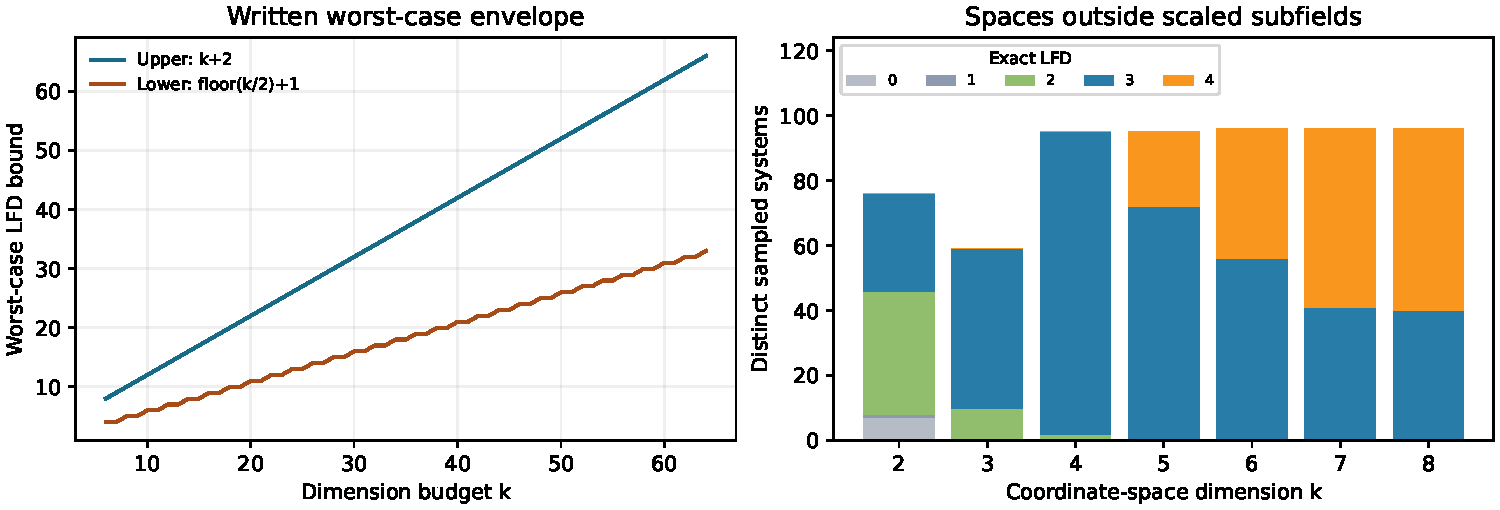
\includegraphics[width=\linewidth]{figures/arbitrary-bases.pdf}
\caption{Left: written bounds on the worst-case dimension-budget quantity,
not exact values. Right: exact LFD histogram by dimension for the new seeded
systems outside the scaled-subfield class. No population inference is made.}
\end{figure}

The data store algebraic tuples, rational coordinate tuples and unordered
multisets separately. For example, 167 order-two cases have polynomial
solutions but only 141 have rational coordinate decompositions; all 222
planted cases pass their rational existence checks. Independent relation
rank remains unknown. The samples cannot prove a constant-four universal
bound, which the structured growing family already excludes.

The separate existing artifact contains 1,803 geometric cases / 1,474
distinct systems with $m=2,\ldots,9$, all now exact after resolving 29 earlier
caps. It also contains 587 scaled-subfield/dilation cases and inverse-model
traces through $n=12$. These campaigns have overlapping geometry and
different presentations; their counts are not added as independent samples.
The original prime-field model experiments did not establish a net decrease
in measured useful-relation collection cost.

\section{Related work and verification boundary}
Huang, Kosters, Yang and Yeo established the LFD and Weil-descent framework
used here~\cite{hkyy}. Caminata and Gorla compare LFD with solving degree
and homogeneous invariants~\cite{cg}. Moore coordinates and cyclic
Frobenius chains are standard descent machinery, not new constructions.
Gorla, Mueller and Petit give improved LFD bounds for univariate fake Weil
descent and HFE systems~\cite{gmp}, especially Section 6, Theorem 11 and
Corollary 1. Their input is a univariate system with field equations; a
direct application to this two-variable inverse presentation requires a
degree-budget-preserving reduction, not just a parameterization by inversion.
Their result is not an exact calculation for the presentation here. This
distinction does not establish priority for our consequence.

Preparata's cyclic nonadjacent representation theorem already supplies
the odd uniqueness and even exceptional patterns~\cite{preparata}.
Standard signed-digit minimality is also discussed by Bosma~\cite{bosma}.
The candidate contribution is the explicit ordinary iterated-closure budget,
full lower obstruction, and its curve/base specialization. General FFD/LFD
separation, ECDLP descent applications, subfield factor bases, and CAS proof
certification are established research topics. The repository's source-level
novelty audit records additional overlapping work and which primary texts
were read. An exact novelty claim requires independent specialist review.

The pinned Lean 4.19.0/mathlib artifact audits 513 declarations (424 when this draft was first written) without
project axioms, proof placeholders or native-decide overrides. Among the
checked components are the ordinary closure definitions, degree-safe affine
transport, local-to-global reduction theorem, scalar binary fiber bounds,
bounded cyclic carries constructed from modular equality, their rigidity,
local degree-three identities, and the all-length even product bridge.
Additional checked links prove arbitrary-dimensional coordinate and Frobenius
identities, invertibility of the actual Moore matrix, both directions of
finite coefficient-field extension for full closures and exact LFD, and
exact affine/input transport with explicit budgets. The main normalization,
coefficient lower obstruction, final Moore input-filtration specialization
and arbitrary-space selector specialization remain written proofs.
Counting checked supporting declarations does not make
Theorems~\ref{thm:uniform} and \ref{thm:inverse} fully kernel-checked.
Separate kernel results include all-$k$ prime two-summand FFD classification
and lower bounds for all-length one-bit split systems; neither supplies
universal larger-$m$ arbitrary-base sharpness.

\section{Reproduction and unresolved questions}
The original source package included this manuscript, figures, exact data, source/data SHA256 manifests, pinned formal sources and audit logs. Of its scripts, only \texttt{verify\_\allowbreak lean\_\allowbreak fall\_\allowbreak degrees.py} is in the public repository, together with the formal sources; the commands below, other than that one, refer to the original package and do not run from the public repository. From the original package:
\begin{verbatim}
python scripts/reproduce_ic_paper.py --lake /path/to/lake
\end{verbatim}
This command runs the full proof-component/data/paper pipeline in an isolated
source copy, including fresh baseline and frontier arithmetic. The report
lists the main theorem's open formal obligations. Adding
\texttt{--require-complete-proof} makes the command exit with failure status
two while these obligations remain open. It does not obtain independent review.
Individual components can also be run directly:
\begin{verbatim}
python scripts/build_ic_paper.py
python scripts/run_ic_arbitrary_bases.py --check-only
python scripts/verify_ic_positive_naf.py --check-only
python scripts/verify_ic_inverse_parity.py
python scripts/run_ic_inverse_subfields.py
python scripts/verify_ic_binary_m2_uniform.py
python scripts/verify_ic_research_artifact.py --replay-inverse-traces
python scripts/verify_lean_fall_degrees.py --lake /path/to/lake
\end{verbatim}
The last command requires the pinned Lean toolchain and mathlib dependencies;
they and copyrighted literature downloads are excluded from the source zip.
Building the PDF requires pdfLaTeX and matplotlib. The new positive-word
check exhausts signed words through length 12 and compares all minimum-weight
representations; it supports Lemma~\ref{lem:positive}, rather than proving
its universal statement computationally.

Outstanding mathematical questions include the exact worst-case constants,
sharp values for unstructured individual spaces and arbitrary targets,
and larger-$m$ systems with unrestricted finite partial sums. Independent
proof review, publication novelty, authorship and venue metadata are not
settled by these experiments or formal components. This manuscript is an
internal review package, not a claim of submission readiness.

\begin{thebibliography}{9}
\bibitem{hkyy} M.-D. A. Huang, M. Kosters, Y. Yang and S. L. Yeo.
\emph{On the last fall degree of zero-dimensional Weil descent systems}.
Journal of Symbolic Computation 87 (2018), 207--226.
\href{https://doi.org/10.1016/j.jsc.2017.08.002}{doi:10.1016/j.jsc.2017.08.002}.
\bibitem{cg} A. Caminata and E. Gorla.
\emph{Solving degree, last fall degree, and related invariants}.
Journal of Symbolic Computation 114 (2023), 322--335.
\href{https://arxiv.org/abs/2112.05579}{arXiv:2112.05579}.
\bibitem{gmp} E. Gorla, D. Mueller and C. Petit.
\emph{Stronger bounds on the cost of computing Gr\"obner bases for HFE systems}.
 Journal of Symbolic Computation 109 (2022), 386--398.
\href{https://doi.org/10.1016/j.jsc.2020.07.011}{doi:10.1016/j.jsc.2020.07.011}.
\bibitem{preparata} F. P. Preparata.
\emph{On the Representation of Integers in Nonadjacent Form}.
SIAM Journal on Applied Mathematics 21(4) (1971), 630--635.
\href{https://doi.org/10.1137/0121067}{doi:10.1137/0121067}.
\bibitem{bosma} W. Bosma.
\emph{Signed bits and fast exponentiation}.
Journal de Th\'eorie des Nombres de Bordeaux 13(1) (2001), 27--41.
\href{https://jtnb.centre-mersenne.org/article/JTNB_2001__13_1_27_0.pdf}{Author text}.
\end{thebibliography}
\end{document}
